% 2010 年浙江卷理科第 19 题：投球管道。
% 来源 PDF：普通高考/2010/2010浙江理.pdf，SHA-256 c61b26c8cab009d567644272afc34d81e3174ffa90244c333ecfb27d61034a00。
% 原页：第 1 页（A3 三栏）第 3 栏下部，书页码 639。
% 重绘依据：M 下第一叉口分左右；左支再分叉，左外支直达 C，内支入中；右支同理，
%   右外支直达 B，内支入中；两内支在中部汇合后再平分，左入 C、右入 A。
%   出口自左至右为 C、A、B；管道以双线表示，与原页拓扑一致。
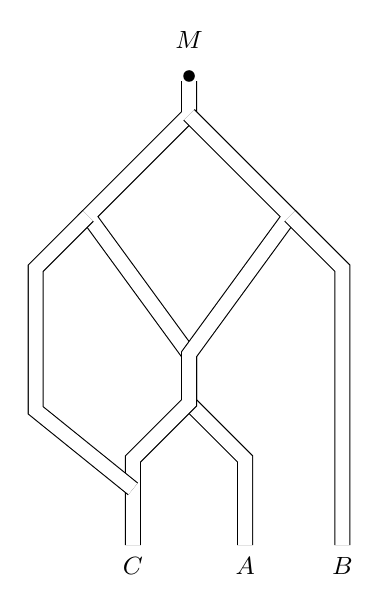
\begin{tikzpicture}[scale=0.95, every node/.style={inner sep=1.5pt, font=\small},
  pipe/.style={double, double distance=5pt, line width=0.4pt}]

  % M 至第一叉口，及左内支→中部→右叉口→A 的连续通道
  \draw[pipe] (0,7.35) -- (0,6.9) -- (-1.35,5.55) -- (0,3.7) -- (0,3.05)
    -- (0.75,2.3) -- (0.75,1.15);
  % 右内支→中部→左叉口→C 的连续通道
  \draw[pipe] (0,6.9) -- (1.35,5.55) -- (0,3.7) -- (0,3.05)
    -- (-0.75,2.3) -- (-0.75,1.15);
  % 左外支到 C
  \draw[pipe] (-1.35,5.55) -- (-2.05,4.85) -- (-2.05,2.95) -- (-0.75,1.9);
  % 右外支到 B
  \draw[pipe] (1.35,5.55) -- (2.05,4.85) -- (2.05,1.15);

  \node[below] at (-0.75,1.05) {$C$};
  \node[below] at (0.75,1.05) {$A$};
  \node[below] at (2.05,1.05) {$B$};

  % 投球点 M
  \fill (0,7.42) circle (2.2pt);
  \node[above] at (0,7.72) {$M$};
\end{tikzpicture}
